\section{La transform\'{e}e en $z$}
L'objet de cette section est de d\'{e}finir la transform\'{e}e en $z$, et de voir sous quelles conditions elle converge.
\subsection{Transformée en $z$ directe}
\begin{definition}[Transformée en $z$]
\label{def:transformee}
La transform\'{e}e en $z$ d'une suite $\sequence{u}[n][\zset]$ est d\'{e}finie comme la s\'{e}rie $U(z)$ calcul\'{e}e comme suit:
\begin{equation}
\label{eq:definition-transformee}
U(z)=\sum_{n=-\infty}^{\infty} u_n z^{-n}
\end{equation}
o\`{u} $z$ est une variable complexe.
\end{definition}
On appelle encore \eqref{eq:definition-transformee} la transform\'{e}e directe, car c'est la relation qui permet d'obtenir $U(z)$ \`{a} partir de $\sequence{u}[n][\zset]$. Cette transfomée est bilatérale. L'op\'{e}ration inverse porte le nom de transformation inverse.

Comme cette transformation est une s\'{e}rie infinie, elle n'existe que pour les valeurs de $z$ pour lesquelles cette s\'{e}rie converge. La r\'{e}gion de convergence (RC) est l'ensemble des valeurs de $z$ pour lesquelles la s\'{e}rie prend une valeur finie. Dès lors, \emph{toute transform\'{e}e en $z$} doit \^{e}tre accompagnée de la région du plan complexe sur laquelle elle converge. Pour d\'{e}terminer la r\'{e}gion de convergence, on utilise le crit\`{e}re de Cauchy sur la convergence des s\'{e}ries entières. Rappelons que la s\'{e}rie à termes positifs
$ \sum_{n=0}^{\infty} v_n$ converge si
\begin{equation}
\label{eq:critere-cauchy}
\limsup_{n\rightarrow\infty} v_{n}^{1/n}<1 \eqsp.
\end{equation}
Pour appliquer le crit\`{e}re de Cauchy, on d\'{e}compose la s\'{e}rie en deux s\'{e}ries:
$$
U(z)\ =\ \sum_{n=-\infty}^{-1} u_n z^{-n}+\sum_{n=0}^{\infty} u_n z^{-n} = U_1(z) + U_2(z) \eqsp.
$$
L'application du crit\`{e}re de Cauchy \`{a} la s\'{e}rie $U_{2}(z)$ m\`{e}ne \`{a}
\begin{align*}
\limsup_{n\rightarrow\infty}| u_n z^{-n}|^{1/n}\ <\ 1  \quad \Rightarrow \quad
\limsup_{n\rightarrow\infty}| u_n |^{1/n}\ <\ |z|
\end{align*}
En appelant $R_{-}$ la limite
\begin{equation}
\label{eq:definition-R-}
R_{-}=\limsup_{n\rightarrow\infty}|u_n|^{1/n}
\end{equation}
la s\'{e}rie $U_{2}(z)$ converge sur la couronne $\ensemble{z \in \cset}{|z|>R_{-}}$.
Pour ce qui est de la s\'{e}rie $U_{1}(z)$ , apr\`{e}s un changement de variable, on a
$$
U_{1}(z)\ =\ \sum_{n=-\infty}^{-1} u_n z^{-n} =\ \sum_{n=1}^{\infty} u_{-n} z^{n}
$$
On a convergence si
\begin{align*}
\limsup_{n\rightarrow\infty}|u_{-n} z^{n}|^{1/n}\ <\ 1 \quad \Rightarrow \limsup_{n\rightarrow\infty}|u_{-n}|^{1/n}|z|\ <\ 1
\end{align*}
et donc la série $U_1(z)$ converge sur le disque
\begin{equation}
\label{eq:definition-R+}
|z|\ <\ \left\{ \lim_{n\rightarrow\infty}|u_{-n}|^{1/n} \right\}^{-1}=R+
\end{equation}
En toute g\'{e}n\'{e}ralit\'{e}, une s\'{e}rie converge donc  dans un anneau du plan complexe  donn\'{e} par
$$
R_{-}<|z|<R+
$$
Lorsque $R+\leq R_{-}$, le domaine de convergence est vide est la transformée en $z$ de la suite n'est alors pas défini.

La suite $U_{2}(z)$ repr\'{e}sente la transform\'{e}e en $z$ d'une \emph{suite causale}: les seules valeurs non-nulles de la suite
correspondent aux indices positifs. La transformée en $z$ d'une suite causale converge \`{a} l'ext\'{e}rieur d'un cercle de rayon $R_{-}$ donn\'{e} par \eqref{eq:definition-R-}.

La suite $U_{1}(z)$ repr\'{e}sente la transform\'{e}e en $z$ d'une suite anti-causale, c'est-\`{a}-dire ne comportant des \'{e}l\'{e}ments que pour les valeurs n\'{e}gatives de l'indice. En g\'{e}n\'{e}ral, une suite anti-causale converge \`{a} l'int\'{e}rieur d'un cercle de rayon $R_+$donn\'{e} par \eqref{eq:definition-R+}. Quand une suite est \`{a} dur\'{e}e limit\'{e}e, sa transform\'{e}e est donn\'{e}e par
\begin{equation}
\label{eq:z-duree-limitee}
U(z)=\sum_{n=n_{1}}^{n_{2}} u_n z^{-n}
\end{equation}
Pour autant que dans l'intervalle $[n_{1},\ n_{2}]$ le module de chaque \'{e}l\'{e}ment de la suite soit fini, la s\'{e}rie converge pour toutes les valeurs de $z$, sauf \'{e}ventuellement en $z=0$ ou $|z|\rightarrow\infty$. Les cas suivants peuvent \^{e}tre distingu\'{e}s:
\begin{enumerate}
\item si $n_{1}$ et $n_{2}$ sont positifs, on n'a pas convergence pour $z=0$ car les termes $z^{-n}$ divergent pour les $n$ positifs.
\item  si $n_{1}$ est n\'{e}gatif et $n_{2}$ est positif, on n'a pas convergence ni pour $z=0$ ni $|z|\rightarrow\infty$.
\item si $n_{1}$ et $n_{2}$ sont n\'{e}gatifs, on n'a pas convergence pour $|z|\rightarrow\infty$.
\end{enumerate}
Consid\'{e}rons les exemples suivants:
\begin{enumerate}
\item $u_n=\delta_n$ : la d\'{e}finition fournit directement $U(z)=1$. La transform\'{e}e existe partout.
\item $u_n=1$ si $n \geq 0$ et $u_n=0$ sinon :
$$
U(z)=\sum_{n=0}^{\infty}z^{-n}=\frac{1}{1-z^{-1}}
$$
pour $R_{-}=\displaystyle \lim_{n\rightarrow\infty}1^{1/n}=1^{1}$
\item $u_n=a^{n}$ pour $n \geq 0$, $u_n=0$ sinon
\begin{equation}
\label{eq:z-exponentiel}
\sum_{n=0}^{\infty}a^{n}z^{-n}=\sum_{n=0}^{\infty}(az^{-1})^{n}=\frac{1}{1-az^{-1}}
\end{equation}
avec un domaine de convergence $|z|>|a|$.
\item $u_n = \rme^{ 2 \rmi \pi \nu_0 n}$
$$
U(z)=\sum_{n=0}^{\infty}\rme^{2 \rmi \pi \nu_0 n}z^{-n}=\sum_{n=0}^{\infty}( \rme^{2 \rmi \pi \nu_0} z^{-1})^{n}=\frac{1}{1- \rme^{2 \rmi \pi \nu_0} z^{-1}}
$$
avec un domaine de convergence $|z|>1$.
\item La suite $u_n= a^n$ pour $n \in \zset$ n'a pas de transformée en $z$.
\end{enumerate}
\subsection{Transformée inverse}
Pour inverser une transform\'{e}e en $z$, on peut s'aider utilement du \emph{théorème de Cauchy} qui \'{e}tablit que
\begin{equation}
\label{eq:cauchy}
\frac{1}{2\pi \rmi}\oint_{\Gamma}z^{l-1}\rmd  z= \begin{cases} 1 & l= 0 \\ 0 & \text{sinon} \end{cases}
\end{equation}
o\`{u} $\Gamma$ est un contour qui entoure l'origine du plan et est parcouru dans le sens trigonométrique. En reprenant la d\'{e}finition de la transform\'{e}e en $z$ donn\'{e}e par \eqref{eq:definition-transformee}, en multipliant les deux membres par $z^{l-1}$ et en int\'{e}grant le long d'un contour entourant l'origine et appartenant au domaine de convergence, on trouve
\begin{align*}
\oint_{\Gamma}U(z)z^{l-1}\rmd z\ &=\ \oint_{\Gamma}\sum_{n=-\infty}^{\infty} u_n z^{-n+l-1}\rmd z \\
&=\ \sum_{n=-\infty}^{\infty} u_n \oint_{\Gamma}z^{-n+l-1}\rmd z
\end{align*}
o\`{u} l'interversion de l'int\'{e}grale et de la somme est licite compte tenu du fait que l'on op\`{e}re dans la zone de convergence de la transform\'{e}e. En utilisant le th\'{e}or\`{e}me de Cauchy \eqref{eq:cauchy}, on a finalement
\begin{equation}
\label{eq:inverse-z}
u_n=\frac{1}{2\pi \rmi}\oint_{\Gamma} U(z)z^{n-1}\rmd z
\end{equation}
avec les conditions d\'{e}j\`{a} \'{e}nonc\'{e}es \`{a} propos du contour d'int\'{e}gration.

L'\'{e}valuation de l'int\'{e}grale dans le plan complexe se fait \`{a} l'aide du th\'{e}or\`{e}me des r\'{e}sidus, qui \'{e}tablit que l'int\'{e}grale le long d'un contour est donn\'{e} par la somme des r\'{e}sidus de la fonction \`{a} int\'{e}grer, soit ici $U(z)z^{n-1}$, dans le contour $\Gamma$. Le r\'{e}sidu $r_{q}$ \`{a} un p\^{o}le d'ordre $q$ en $z=a$ est donn\'{e} par
\begin{equation}
\label{eq:residu-q}
r_{q}=\lim_{z\rightarrow a}\frac{1}{(q-1)!}\frac{\rmd ^{q-1}}{\rmd z^{q-1}}[U(z)z^{n-1}(z-a)^{q}]
\end{equation}
Pour un p\^{o}le simple $(q=1)$ en $z=a$, l'expression du r\'{e}sidu $r_{1}$ se r\'{e}duit \`{a}
\begin{equation}
\label{eq:residu-simple}
r_{1}=\lim_{z\rightarrow a}[U(z)z^{n-1}(z-a)]
\end{equation}
\begin{example}
Consid\'{e}rons la transform\'{e}e en $z$ donn\'{e}e par
$$
U(z)=\frac{1}{1-z^{-1}}
$$
et le domaine de convergence $|z|>1$. En utilisant la formule d'inversion, on a donc que
\begin{align*}
u_n\ &=\ \frac{1}{2\pi \rmi}\oint_{\Gamma}\frac{z^{n-1}}{1-z^{-1}}\rmd z
&=\ \frac{1}{2\pi \rmi}\oint_{\Gamma}\frac{z^{n}}{z-1}\rmd z
\end{align*}
o\`{u} le contour $\Gamma$ peut \^{e}tre un cercle de rayon plus grand que l'unit\'{e}. Pour $n\geq 0$, on n'a qu'un p\^{o}le d'ordre 1 en $z=1$ qui est entour\'{e} par le contour. Le r\'{e}sidu en ce p\^{o}le est donn\'{e} par $r_{1}$ valant
$$
r_{1}=\lim_{z\rightarrow 1}[z^{n}]=1
$$
On a donc $u_n=1$ pour tout $n \geq 0$. En ce qui concerne $n<0$, on a cette fois un autre p\^{o}le d'ordre $(-n)$ en $z=0$.
L'application de la formule du r\'{e}sidu donne, pour $q=-n$,
$$
 r_{q}=\lim {z\rightarrow 0} \frac{1}{(q-1)!}\frac{\rmd ^{q-1}}{\rmd z^{q-1}}[\frac{1}{z-1}]=-1
$$
autre r\'{e}sidu vaut toujours 1 et la somme donne donc $0$.
Pour \'{e}vi- ter l'\'{e}valuation fastidieuse du r\'{e}sidu en un p\^{o}le d'ordre non \'{e}gal \`{a} un, on peut recourir \`{a} un changement de variable $w=1/z$. On \`{a} d\`{e}s lors que le domaine de convergence devient $|w|<1$, et l'int\'{e}grale \`{a} \'{e}valuer devient
\begin{align*}
u_n\ &=\ \frac{1}{2\pi j}\oint_{\Gamma}\frac{z^{n}}{z-1}\rmd  z \\
     &=\ \frac{1}{2\pi j}\oint_{\Gamma^{-}}\frac{w^{-n}}{w^{-1}-1}\frac{(-1)}{w^{2}}\rmd w\\
     &=\ \frac{1}{2\pi j}\oint_{\Gamma+}\frac{w^{-n-1}}{1-w}\rmd  w =\ 0
\end{align*}
o\`{u} le contour $\Gamma^{-}$ peut \^{e}tre un cercle de rayon inf\'{e}rieur \`{a} l'unit\'{e} et parcouru dans le sens anti-trogonométrique (à cause du changement de variable). Le contour $\Gamma^{+}$ est parcouru dans le sens trigonométrique et compense le signe -. Pour $n<0$, on n'a pas de p\^{o}le en $0$. Le seul p\^{o}le est en $w=1$ mais n'est pas entour\'{e} par le domaine d'int\'{e}gration qui doit appartenir au domaine de convergence, soit $|w|<1$. Aucun p\^{o}le n'est donc entour\'{e} et la somme des r\'{e}sidus est nulle.
\end{example}
\subsection{D\'{e}compositions en fractions simples}
En utilisant d'ores et d\'{e}j\`{a} la propri\'{e}t\'{e} de lin\'{e}arit\'{e} de la transform\'{e}e en $z$, qui sera vue plus loin, on peut d\'{e}composer une fonction de forme compliqu\'{e}e en une somme de fonctions simples, et prendre la transform\'{e}e inverse de chacun des \'{e}l\'{e}ments. Comme on le verra, de nombreux syst\`{e}mes requi\`{e}rent l'\'{e}tude de transform\'{e}es du type
\begin{equation}
\label{eq:definition-U}
U(z)=P(z)/Q(z)
\end{equation}
o\`{u} $P$ et $Q$ sont des polyn\^{o}mes en $z$ ou $z^{-1}$. On peut alors d\'{e}composer $U(z)$ en fractions simples et obtenir la transform\'{e}e inverse par la somme des transform\'{e}es inverses. La transform\'{e}e peut se mettre sous la forme
$$
U(z)=S(z)+P_{0}(z)/Q(z)
$$
o\`{u} le degr\'{e} de $P_{0}(z)$ est inf\'{e}rieur \`{a} celui de $Q(z)$ . En fait, $S(z)$ et $P_{0}(z)$ sont respectivement le quotient et le reste de la division de $P$ par $Q$. Si le degr\'{e} de $P$ est inf\'{e}rieur \`{a} celui de $Q$, le quotient $S$ est nul.

Lorsque les racines $p_{i}$ de $Q(z)$ , appel\'{e}es p\^{o}les sont simples, on peut mettre le quotient sous la forme
\begin{equation}
\label{eq:decomposition-pole-simple}
P_{0}(z)/Q(z)=\sum_{i=1}^{N}\frac{\alpha_{i}}{z-p_{i}}
\end{equation}
Pour obtenir les poids $\alpha_{i}$, il suffit d'effectuer le calcul suivant:
$$
\alpha_{i}=[(z-p_{i})P_{0}(z)/Q(z)]_{z=p_{i}} \eqsp.
$$
Si un p\^{o}le $p_{n}$ est d'ordre $q>1$, la d\'{e}composition prend la forme
$$
P_{0}(z)/Q(z)=\sum_{i=1,\neq n}^{N}\frac{\alpha_{i}}{z-p_{i}}+\sum_{j=1}^{q}\frac{\beta_{j}}{(z-p_{n})^{j}}
$$
avec
$$
\beta_{j}=\frac{1}{(q-j)!}\frac{\mathrm{d}^{q-j}}{\mathrm{d}z^{q-j}}[(z-p_{n})^{j}P_{0}(z)/Q(z)]_{z=p_{n}}\text{   }(2.40)
$$
En r\'{e}alit\'{e}, il est plus int\'{e}ressant d'obtenir des fractions o\`{u} $z^{-1}$ apparaît au
d\'{e}nominateur, car les fractions dans ce cas correspondent directement \`{a} des
transform\'{e}es connues. D\`{e}s lors, tout ce qui vient d'\^{e}tre dit est appliqu\'{e} pour
des polyn\^{o}mes en $z^{-1}$ et non pas en $z$.

\begin{example}
Consid\'{e}rons la transform\'{e}e donn\'{e}e par
$$
U(z)=\frac{1}{1-3z^{-1}+2z^{-2}}
$$
pour $|z|>2$. Comme nous consid\'{e}rons que la variable est $z^{-1}$, le degr\'{e} du num\'{e}rateur est bien inf\'{e}rieur \`{a} celui du d\'{e}nominateur.
Les p\^{o}les sont donn\'{e}s par $z^{-1}=1$ et $z^{-1}=0.5$. On recherche donc une d\'{e}composition en fractions simples du type
\begin{align*}
U(z)\ &= \frac{0.5}{(z^{-1}-1)(z^{-1}-0.5)} \\
      &=\ \frac{\alpha_{1}}{z^{-1}-1}+\frac{\alpha_{2}}{z^{-1}-0.5}
\end{align*}
On trouve en utilisant ce qui a \'{e}t\'{e} vu pr\'{e}c\'{e}demment,
$$
U(z)=\frac{1}{z^{-1}-1}+\frac{-1}{z^{-1}-0.5}
$$
D\`{e}s lors,
$$
U(z)=\frac{2}{1-2z^{-1}}-\frac{1}{1-z^{-1}}
$$
et il est possible d'identifier ces fractions au r\'{e}sultat obtenu en \eqref{eq:z-exponentiel}. On trouve de ce fait
$$
u_n=2\times 2^{n} \1_{\nset}(n) - \1_{\nset}(n)=(2^{n+1}-1) \1_{\nset}(n) .
$$
Si on avait consid\'{e}r\'{e} les polyn\^{o}mes comme des fonctions de $z$, on aurait eu
\begin{align*}
U(z) &=\ \frac{1}{1-3z^{-1}+2z^{-2}} \\
     &=\ \frac{z^{2}}{z^{2}-3z+2}\\
     &=\ 1+\frac{3z-2}{z^{2}-3z+2}\\
     &=\ 1+\frac{3z-2}{(z-2)(z-1)}\\
     &=\ 1+\frac{4}{(z-2)}+\frac{-1}{(z-1)}\\
     &=\ 1+\frac{4z^{-1}}{(1-2z^{-1})}-\frac{1}{(1-z^{-1})}
\end{align*}
En s'aidant de la propri\'{e}t\'{e} de d\'{e}calage qui sera vue plus loin, on a que
$$
u_n=\delta_n +4\times 2^{n-1} \1_{\nset}(n-1)-\1_{\nset}(n-1) \eqsp.
$$
Cette forme est moins concise que la pr\'{e}c\'{e}dente.
\end{example}
\subsection{Propri\'{e}t\'{e}s de la transform\'{e}e en $z$}
\subsubsection{Lin\'{e}arit\'{e}}
La lin\'{e}arit\'{e} de la transformation signifie que la transform\'{e}e d'une suite obtenue par combinaison lin\'{e}aire d'autres suites n'est rien d'autre que la combinaison lin\'{e}aire des transform\'{e}es correspondantes. Sidonc
$$
u_n=a x_n +b y_n
$$
alors
\begin{align*}
U(z)\ &=\ \sum_{n=-\infty}^{\infty} u_n z^{-n} =\ a\ \sum_{n=-\infty}^{\infty}x_{n} z^{-n}+b\sum_{n=-\infty}^{\infty} y_n z^{-n} \\
&=\ a\ X(z)+bY(z)
\end{align*}
La r\'{e}gion de convergence est au moins l'intersection des r\'{e}gions associ\'{e}es \`{a} $X(z)$ et $Y(z)$ car la combinaison lin\'{e}aire peut introduire des z\'{e}ros qui compensent certains p\^{o}les.

\subsubsection{D\'{e}calage et transform\'{e}e bilat\'{e}rale}
Soit
$$
v_n =u_{n-n_{0}}
$$
La transform\'{e}e en $z$ de $\sequence{v}[n][\zset]$ est donn\'{e}e par
\begin{align*}
V(z) &=\ \sum_{n=-\infty}^{\infty} v_n z^{-n} \\
     &=\ \sum_{n=-\infty}^{\infty}u_{n-n_0}z^{-n} \\
     &=\ \sum_{m=-\infty}^{\infty}u_n z^{-(m+n_{0})} \\
     &=\ z^{-n_{0}} U(z)
\end{align*}
Le domaine de convergence est le m\^{e}me celuide $U(z)$ sauf que si $n_{0}$ est positif (resp. n\'{e}gatif), on a un p\^{o}le en $0$ (resp. $ z\rightarrow\infty$). Il peut y avoir des compensations de z\'{e}ros ou p\^{o}les.

Multiplier une transform\'{e}e en $z$ par $z^{-1}$ revient donc \`{a} retarder la suite d'une unit\'{e} (p\'{e}riode d'\'{e}chantillonnage). On se r\'{e}f\`{e}re souvent \`{a} $z^{-1}$ comme op\'{e}rateur de retard unit\'{e}.

La propri\'{e}t\'{e} de d\'{e}calage permet de traiter les \'{e}quations aux diff\'{e}rences vues pr\'{e}c\'{e}demment. A partir de
$$
v_n = u_n - \sum_{k=1}^p b_k u_{n-k}
$$
on trouve par transformation en $z$,
\begin{align*}
V(z) &=\ U(z)- \sum_{k=1}^p b_{k}z^{-k}V(z)
\end{align*}
ce qui implique que
\[
V(z) =\frac{U(z)}{1+ \sum_{k=1}^p b_{k}z^{-k}}
\]
Il faut faire attention toutefois avec ce calcul "formel" que les régions de convergence de $U(z)$ et de $1/ (1 + \sum_{k=1}^p b_k z^{-k})$ soient compatibles. Nous reviendrons sur cet aspect plus loin dans l'exposé.
\subsubsection{D\'{e}calage et transform\'{e}e unilat\'{e}rale}
Dans le cas unilat\'{e}ral, il faut \^{e}tre plus prudent dans ce que l'on \'{e}crit. La transformée unilatérale de la suite $\sequence{u}[n][\zset]$ est donnée par
\begin{equation}
\label{eq:transformee-unilaterale}
\tilde{U}(z)= \sum_{k=0}^\infty u_k z^{-k}\eqsp.
\end{equation}
Notons que nous ne calculons la somme que pour les indices positifs ! Le rayon de convergence de la transfomrmée monolatérale est une couronne
donnée ${z \in \cset}{|z| \geq \limsup_{n \to \infty} |u_n|^{1/n}}$.
Si on pose $v_n=u_{n-1}$ , la transform\'{e}e bilat\'{e}rale est calcul\'{e}e par
\begin{align}
\nonumber
\tilde{V}(z)\ &=\ \sum_{n=0}^{\infty}v_nz^{-n} \\
\nonumber
&=\ \sum_{n=0}^{\infty}u_{n-1}z^{-n} \\
\nonumber
&=\ z^{-1}\sum_{m=-1}^{\infty} u_m z^{-m} \\
\nonumber
&=\ z^{-1}[u_{-1} z+\tilde{U}(z)] \\
&=\ u_{-1}+z^{-1}\tilde{U}(z)
\label{eq:decalage-unilateral}
\end{align}
On voit donc qu'un d\'{e}calage vers la droite permet de faire appara\^{i}tre des \'{e}l\'{e}ments qui ne sont pas pris en consid\'{e}ration par la transformation unilatérale de d\'{e}part. Cette propri\'{e}t\'{e} permet de prendre en compte les conditions initiales non nulles.
Soit
\[
v_n=u_n+av_{n-1}\
\]
avec $v_{-1}=K$ et une excitation $u_n=\rme^{2 \rmi \pi \nu_0 n} \1_{\nset}(n)$ . En vertu de \eqref{eq:decalage-unilateral}
la transform\'{e}e en $z$ donne
\begin{align*}
\tilde{V}(z)\ &=\ \tilde{U}(z)+av_{-1}+az^{-1}\tilde{U}(z) \\
&=\ \frac{\tilde{U}(z)+av_{-1}}{1-az^{-1}} \\
&=\ \frac{aK}{1-az^{-1}}+\frac{1}{(1-az^{-1})(1- \rme^{2 rmi \pi \nu_{0}}z^{-1})} \\
& =\ \frac{aK}{1-az^{-1}}+\frac{1}{(1-\rme^{2 \rmi \pi nu_{0}}/a)(1-az^{-1})}
+ \frac{1}{(1-a/\rme^{2 \rmi \pi \nu_{0}})(1-\rme^{2 rmi \pi \nu_{0}}z^{-1})} \\
&=\ \frac{aK}{1-az^{-1}}+\frac{a}{(a-\rme^{2 \rmi \pi \nu_{0}})(1-az^{-1})}
+\ \frac{\rme^{2 \rmi \pi \nu_{0}}}{(\rme^{2 \rmi \pi \nu_{0}}-a)(1-\rme^{2 \rmi \pi\nu_{0}}z^{-1})}
\end{align*}
De ce fait, en utilisant les transform\'{e}es inverses d\'{e}j\`{a} \'{e}tablies, on
trouve
\[
v_n=\1_\nset(n)[a^{n+1}K+\frac{a^{n+1}}{a-\rme^{2 \rmi \pi \nu_{0}}}-\frac{\rme^{2 \rmi \pi \nu_{0}(n+1)}}{a-\rme^{2 \rmi \pi \nu_{0}}}]\
\]
La premi\`{e}re partie de la r\'{e}ponse correspond \`{a} la r\'{e}ponse libre, c'est-
\`{a}-dire l'\'{e}volution du syst\`{e}me sous l'effet des conditions initiales.
La seconde partie correspond \`{a} la partie transitoire de la r\'{e}ponse
forc\'{e}e. La troisi\`{e}me partie correspond \`{a} la r\'{e}ponse de r\'{e}gime de la
r\'{e}ponse forc\'{e}e.

On peut bien \'{e}videmment g\'{e}n\'{e}raliser ce qui pr\'{e}c\`{e}de au cas de plusieurs conditions initiales.

%Changement d'\'{e}chelle
%
%Si on effectue un changement de variable complexe $w=az$ o\`{u} $a$ peut \^{e}tre complexe, le domaine de convergence est modffi\'{e} comme suit
%$$
%R_{-}\ <\ |z|<R+
%$$
%$$
%R_{-}\ <\ |w/a|<R+
%$$
%$$
%|a|R_{-}\ <\ |w|<|a|R+\text{   }(2.58)
%$$
%De plus, si la transform\'{e}e en $z$ poss\`{e}de un p\^{o}le en $z=p$, la transform\'{e}e ex- prim\'{e}e \`{a} l'aide de $w$ poss\`{e}de un p\^{o}le en $w=az=ap$. On voit donc qu'un tel changement de variable permet de modffier la position des p\^{o}les, tant en amplitude qu'en phase puisque la multiplication se fait par un complexe.
%
%26
%
%{\it CHAPITRE 2. LA TRANSFORM\'{E}E EN} $Z$
%
%1. si $a$ est r\'{e}el et positif, on rapproche le p\^{o}le de l'origine si $a<1$ et on l'\'{e}loigne si $a>1$.
%
%2. si $a$ est complexe du type $e^{j\theta}$, le p\^{o}le subit une rotation de $\theta$ radians au- tour de l'origine.
%
%On peut se demander quelle est la suite qui correspond \`{a} cette transform\'{e}e dont la variable ind\'{e}pendante a \'{e}t\'{e} modifi\'{e}e. On peut utiliser la transform\'{e}e inverse pour trouver la r\'{e}ponse. On sait que
%$$
%x(n)\ =\ \frac{1}{2\pi j}\oint_{\Gamma}X(z)z^{n-1}\mathrm{d}z
%$$
%$$
%=\ \frac{1}{2\pi j}\oint_{\Gamma}X(w/a)(w/a)^{n-1}\mathrm{d}(w/a)
%$$
%$$
%x(n)a^{n}\ =\ \frac{1}{2\pi j}\oint_{\Gamma}X(w/a)(w)^{n-1}\mathrm{d}w\text{   }(2.59)
%$$
%et donc $x(n)a^{n}$ est la suite correspondant \`{a} $X(z/a)$ . On verra plus loin combien la position des p\^{o}les et z\'{e}ros est importante car elle conditionne la stabilit\'{e} des syst\`{e}mes lin\'{e}aires. Le fait que la modulation par une suite exponentielle permet de modffier les positions des p\^{o}les et z\'{e}ros est donc de premi\`{e}re importance pour rendre, le cas \'{e}ch\'{e}ant, un syst\`{e}me stable.
%
\subsubsection{D\'{e}rivation}
Comme
$$
U(z)=\sum_{n=-\infty}^{\infty}u_{n}z^{-n}
$$
on a aussi
$$
\frac{\mathrm{d}U(z)}{\mathrm{d}z}=\sum_{n=-\infty}^{\infty}(-n)u_{n}z^{-n-1}
$$
Et donc
$$
-z\frac{\mathrm{d}U(z)}{\mathrm{d}z}=\sum_{n=-\infty}^{\infty}nu_{n}z^{-n}
$$
De ce fait, il appara\^{i}t que $-z\mathrm{d}U(z)/\mathrm{d}z$ est la transform\'{e}e de la suite $\{nu_{n}, n \in \zset\}$ .
%
\subsubsection{Convolution}

Cette propri\'{e}t\'{e} est une des plus importantes et justffie \`{a} elle seule l'usage qui est fait de la transform\'{e}e en $z$ pour \'{e}tudier les syst\`{e}mes lin\'{e}aires permanents en temps discret. Si $\sequence{y}[n][\zset]$ est obtenu par convolution de $\sequence{x}[n][\zset]$ et $\sequence{g}[n][\nset]$ , on a que
$$
y_n=\sum_{m=-\infty}^{\infty}x_m\ g_{n-m}
$$
La transform\'{e}e en $z,\ Y(z)$ , de $\sequence{y}[n][\nset]$ est donc obtenue par
\begin{align*}
Y(z)\ &=\ \sum_{n=-\infty}^{\infty} y_n z^{-n} \\
&=\ \sum_{n=-\infty}^{\infty}\sum_{m=-\infty}^{\infty} x_m\ g_{n-m}z^{-n} \\
&=\ [\sum_{m=-\infty}^{\infty} x_m z^{-m}][\sum_{n=-\infty}^{\infty}g_{n-m}z^{-(n-m)}] \\
&=\ X(z)G(z)
\end{align*}
Cette op\'{e}ration est valable pour les valeurs de $z$ appartenant \`{a} l'intersection des domaines de convergence des deux transform\'{e}es.

Consid\'{e}rons un syst\`{e}me lin\'{e}aire et permanent de r\'{e}ponse impulsionnelle
\[
g_n=a^{n} \1_{\nset}(z)
\]
et $|a|<1$ dont le signal \`{a} l'entr\'{e}e est la suite
$$
x_n=b^{n} \1_{\nset}(n)
$$
et $|b|<1$ avec de plus $|b|>|a|$. La sortie $\sequence{y}[n][\nset]$ est obtenue par $y=x * g$ Les transform\'{e}es $X(z)$ et $G(z)$ sont donn\'{e}es par
\begin{align*}
X(z) &=  \frac{1}{1-bz^{-1}} \quad \text{pour $|z|>|b|$} \\
G(z) &=  \frac{1}{1-az^{-1}} \quad \text{pour $|z|>|a|$}
\end{align*}
En vertu de ce qui pr\'{e}c\`{e}de, on a donc pour $|z|>|b|$ qui est donc l'intersection des domaines de convergence,
\begin{align*}
Y(z)\ &=\ G(z)X(z) =\ \frac{1}{1-az^{-1}}\frac{1}{1-bz^{-1}}\\
&=\ \frac{1}{(1-b/a)(1-az^{-1})}+\frac{1}{(1-a/b)(1-bz^{-1})} \\
&=\ \frac{a}{(a-b)(1-az^{-1})}+\frac{b}{(b-a)(1-bz^{-1})}\
\end{align*}
et donc, compte tenu des transform\'{e}es calcul\'{e}es pr\'{e}c\'{e}demment,
$$
y_n=\1_\nset(n)[\frac{a}{(a-b)}a^{n}+\frac{b}{(b-a)}b^{n}]
$$
%Ces calculs sont illu str\'{e}s \`{a} la figure 2.4, pour $a=0.8,\ b=0.9$.
%Sequence $\mathrm{g};\mathrm{a}=0.8$
%\begin{center}
%\includegraphics[width=107.70mm,height=22.31mm]{./Transformee_En_Z_images/image005.eps}
%\end{center}
%$0$ 2 4 6 $\mathrm{S}\mathrm{e}^{8}\mathrm{q}\mathrm{u}\mathrm{e}\mathrm{n}\mathrm{c}\mathrm{e}^{1}\mathrm{x}^{0}\mathrm{b}=0.9^{12}$ 14 16 18
%\begin{center}
%\includegraphics[width=107.70mm,height=22.35mm]{./Transformee_En_Z_images/image006.eps}
%\end{center}
%$0$ 2 4 6 $\mathrm{s}\ominus \mathrm{q}_{\mathrm{U}\ominus\cap \mathrm{c}\mathrm{e}\mathrm{c}\mathrm{o}\mathrm{n}\mathrm{v}\mathrm{o}}^{8\mathrm{l}01}|\mathrm{u}\mathrm{t}\mathrm{i}\mathrm{o}\mathrm{n}^{2}$ 14 16 18
%\begin{center}
%\includegraphics[width=105.33mm,height=25.74mm]{./Transformee_En_Z_images/image007.eps}
%\end{center}
%FIG. 2.4 --Convolution de deux suites $a^{n}u(n)$ et $b^{n}u(n)$ avec $a=0.8$ et $b=0.9$
%
%{\it 2.2. LA TRANSFORM\'{E}E EN} $Z$
%%
%%29
%%
%Produit de suites
%
%Consid\'{e}rons le signal $y(n)$ obtenu par produit de deux autres $x(n)$ et $g(n)$ . La transform\'{e}e en $z$ est donn\'{e}e par
%$$
%Y(z)\ =\ \sum_{n=-\infty}^{\infty}y(n)z^{-n}
%$$
%$$
%=\ \sum_{n=-\infty}^{\infty}x(n)g(n)z^{-n}\text{   }(2.74)
%$$
%En rempla\c{a}ant $x(n)$ par son expression donn\'{e}e par transformation inverse, on a
%$$
%Y(z)\ =\ \sum_{n=-\infty}^{\infty}\frac{1}{2\pi j}\oint_{\Gamma}X(w)w^{n-1}\mathrm{d}wg(n)z^{-n}
%$$
%$$
%=\ \frac{1}{2\pi j}\oint_{\Gamma}[\sum_{n=-\infty}^{\infty}g(n)(z/w)^{-n}]X(w)w^{-1}\mathrm{d}w
%$$
%$$
%=\ \frac{1}{2\pi j}\oint_{\Gamma}G(z/w)X(w)w^{-1}\mathrm{d}w\text{   }(2.75)
%$$
%Le contour doit \^{e}tre choisi dans l'intersection des domaines de convergence. Pour exprimer la transform\'{e}e inverse de $X(w)$ , il faut
%$$
%R_{-,x}<|w|<R_{+,w}\text{   }(2.76)
%$$
%o\`{u} $R_{-,x}$ et $R_{+,x}$ sont les rayons du domaine de convergence de $X(w)$ . Par ailleurs, pour que $G(z/w)$ existe, il faut
%$$
%R_{-,g}<|z/w|<R_{+,g}\text{   }(2.77)
%$$
%D\`{e}s lors,
%
%$|w|R_{-,g} < R_{-,x}R_{-,g} <$
%
%$|z|<|w|R_{+,g}$
%
%$|z|<R_{+,g}R_{+,x}$ (2.78)
%
%Afin de mieux comprendre le r\'{e}sultat donn\'{e} par l'int\'{e}grale, on peut poser $w= ae^{jb}$ et $z=\alpha e^{j\beta}$; d\`{e}s lors
%$$
%Y(\alpha e^{j\beta})=\frac{1}{2\pi}\int_{-\pi}^{\pi}G(\alpha e^{j(\beta-b)}/a)X(ae^{jb})\mathrm{d}b\text{   }(2.79)
%$$
%ce qui fait appara\^{i}tre que le r\'{e}sultat est le produit de convolution continu et p\'{e}riodique de p\'{e}riode $ 2\pi$ des fonctions $X(ae^{jb})$ et $G(\alpha e^{j\beta})$ .
%Valeur initiale
%
%La transform\'{e}e en $zX(z)$ d'une suite causale $x(n)$ est donn\'{e}e par
%$$
%X(z)\ =\ \sum_{n=0}^{\infty}x(n)z^{-n}
%$$
%$$
%=\  x(\mathrm{O})+\frac{x(1)}{z}+\frac{x(2)}{z^{2}}+\frac{x(3)}{z^{3}}+\cdots\text{   }(2.80)
%$$
%En prenant la limite de cette transform\'{e}e lorsque $z$ tend vers l'infini, il reste donc le premier terme. Donc,
%$$
%x(\mathrm{O})=\lim_{z\rightarrow\infty}X(z)\text{   }(2.81)
%$$
%Cette propri\'{e}t\'{e} n'a de sens que pour des valeurs causales.
%
%Soit la suite donn\'{e}e par sa transform\'{e}e vue en 2.70:
%$$
%X(z)=\frac{z^{2}}{(z-a)(z-b)}=\frac{z^{2}}{z^{2}-(a+b)z+ab}\ (2.82)
%$$
%on a que
%$$
%x(\mathrm{O})=\lim_{z\rightarrow\infty}X(z)=1\ (2.83)
%$$
\subsection{Pôles et zéros}
Dans de nombreux cas d'intérêt, la transformée en $z$ est une fraction rationnelle
\begin{equation}
\label{eq:transformee-z-generale}
H(z)= \frac{\prod_{m=1}^N (1 -z_m z^{-1})}{\prod_{n=1}^N (1 - p_n z^{-1})}
\prod^{M}(z-z_{m})
\end{equation}
o\`{u} les $\{ z_{m} \}_{m=1}^M$ sont les \emph{z\'{e}ros}, et les $\{ p_{n} \}_{n=1}^N$ sont les \emph{p\^{o}les}. 
Pour des signaux et systèmes r\'{e}els, ces polyn\^{o}mes sont \`{a} coefficients r\'{e}els, et leurs racines (p\^{o}les et z\'{e}ros) sont soit r\'{e}elles, soit par paires complexes conjugu\'{e}es. 

Consid\'{e}rons  à  titre d'exemple la suite causale  $h_n=a^{n}\1_\nset(n)$ avec $|a|<1$. La transformée en $z$ de cette suite est donnée par
\begin{equation}
\label{eq:definition-U}
H(z)=\frac{1}{1-az^{-1}} = \frac{z}{z-a}
\end{equation}
sur la couronne $\ensemble{z \in \cset}{|z|>|a|}$. Remarquons que $z \mapsto U(z)$ est défini aussi sur le disque $\ensemble{z \in \cset}{|z|< a}$ et donc que la donnée de \eqref{eq:definition-U} sans préciser le domaine de convergence ne permet pas de reconstruire la suite. 
Cette transform\'{e}e poss\`{e}de un z\'{e}ro en $z=z_1=0$ et un p\^{o}le en $z=p_{1}=a$. La \Cref{fig:FigMignotte-1} illustre le cas d'un p\^{o}le
$a$ r\'{e}el. 
\begin{figure}
  \centering
  % Requires \usepackage{graphicx}
  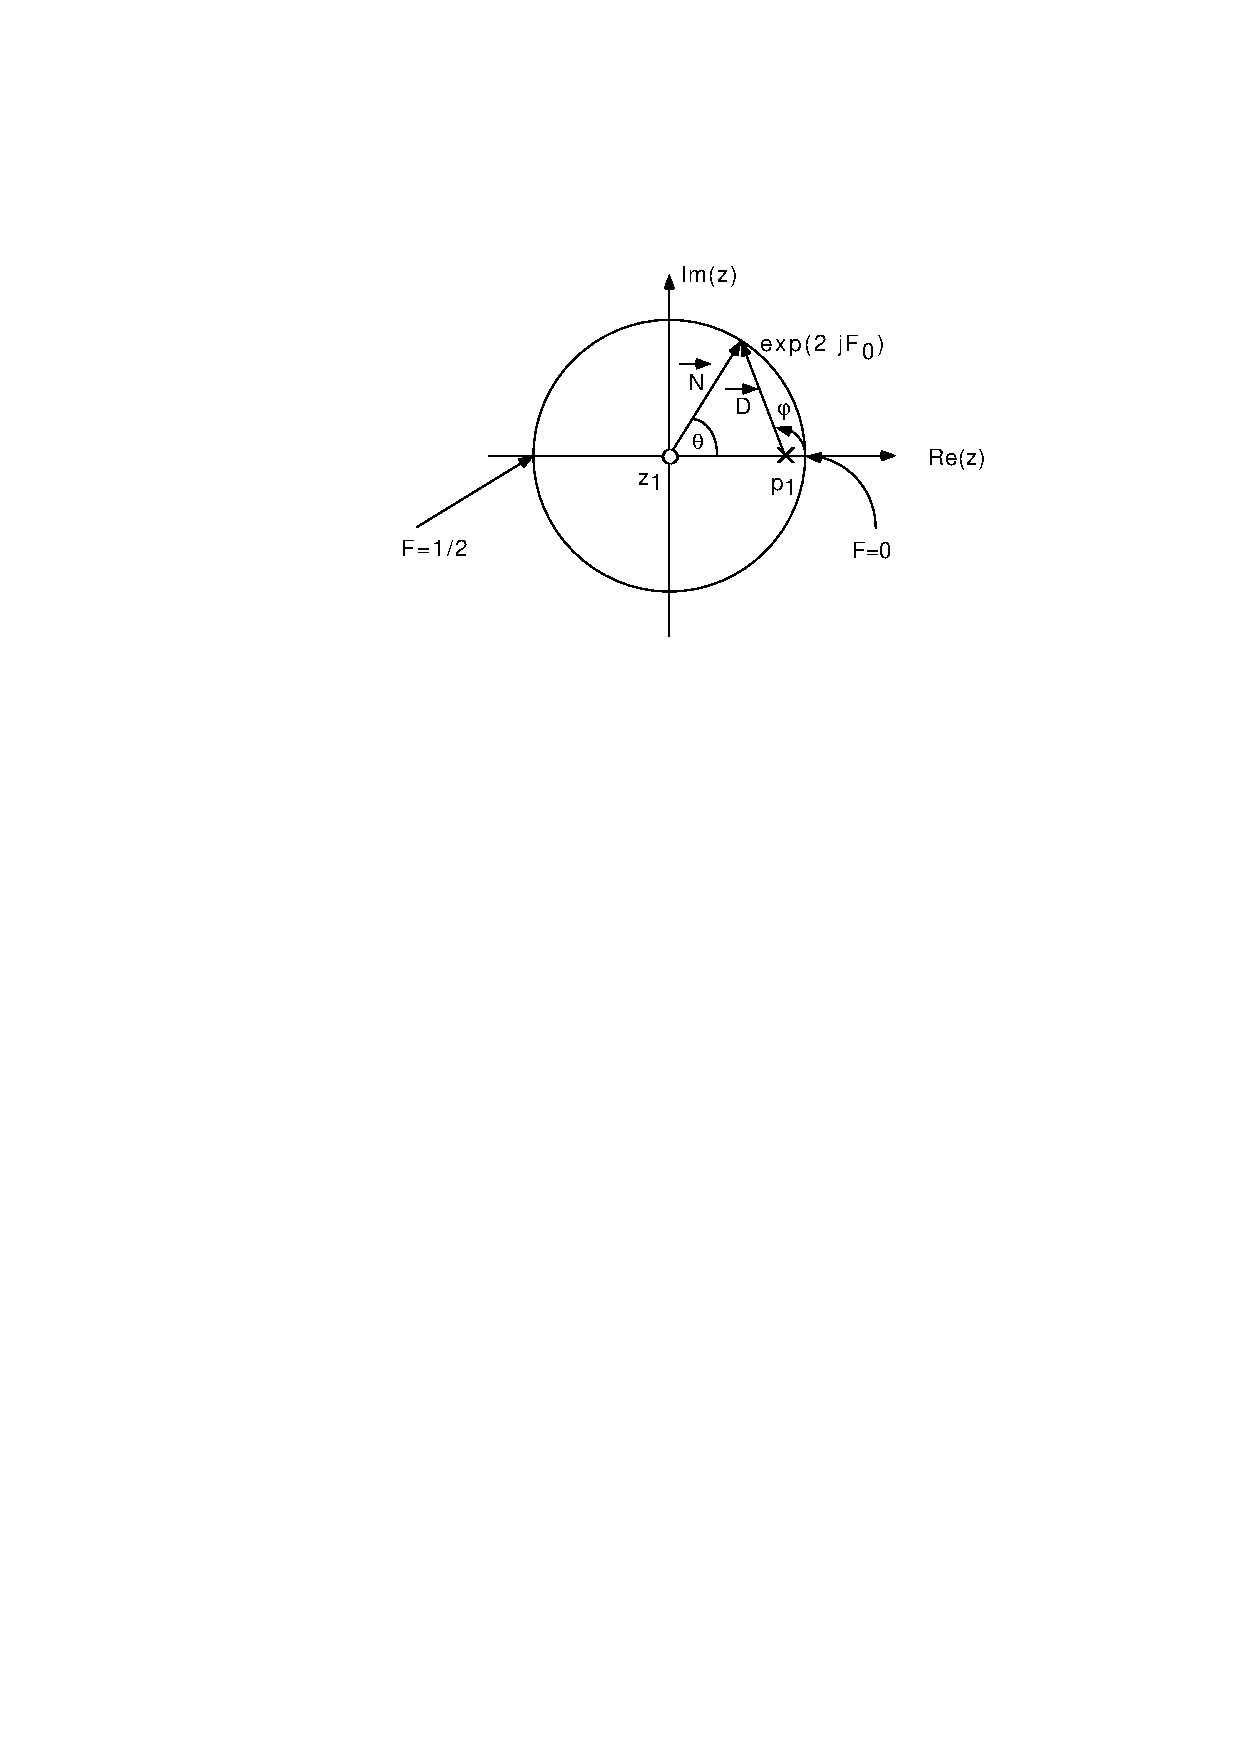
\includegraphics[width=0.6\textwidth]{Figures/FigMignotte-1}\\
  \caption{Réponse en fréquence de $z \mapsto U(z)= 1/(1-az^{-1})$}\label{fig:FigMignotte-1}
\end{figure}

Le calcul de la transform\'{e}e de Fourier requiert d'\'{e}valuer la transform\'{e}e en $z$ sur le cercle de rayon unit\'{e}. Pour une fr\'{e}quence
$F_{0}$, on pose $z=\rme^{2\pi \rmi F_{0}}$ et donc
$$
U(\rme^{2\pi  \rmi F_{0}})=\frac{\rme^{2\pi \rmi F_{0}}}{\rme^{2\pi  \rmi F_{0}}-a}\ 
$$
Le num\'{e}rateur peut \^{e}tre consid\'{e}r\'{e} comme un vecteur joignant l'origine au point $z=e^{2\pi jF_{0}}$. Le d\'{e}nominateur peut \^{e}tre vu comme un
vecteur joignant le point $z=a$ au point $z=\rme^{2\pi  \rmi F_{0}}$ Ces deux vecteurs sont not\'{e}s par $N$ et $B$. Le module de la transform\'{e}e de Fourier est donn\'{e} par le rapport entre longueurs des deux vecteurs.

Quand la fr\'{e}quence change, le module du num\'{e}rateur ne change pas. Par contre le module du d\'{e}nominateur d\'{e}cro\^{i}t lorsque l'on se rapproche d'un p\^{o}le. Plus pr\'{e}cis\'{e}ment, lorsque $2\pi F_{0}$ se rapproche de l'argument d'un p\^{o}le, le d\'{e}nominateur devient petit, et le module de la transform\'{e}e de Fourier devient grand. {\it Le module de la transform \'{e}e de Fourier prend donc des valeurs importantes pour des valeurs de pulsations} $\Omega_{0}=2\pi F_{0}$ {\it proches de l}'{\it argument du  p\^{o}le}. Cette
valeur sera d'autant plus \'{e}lev\'{e}e que le p\^{o}le a un module proche de l'unit\'{e}. On aurait pu tenir le m\^{e}me raisonnement avec les z\'{e}ros, qui occasionnent quant \`{a} eux des valeurs faibles (voire des z\'{e}ros de transmission) de la transform\'{e}e de Fourier. Ici pour $F_{0}=0$, le module du d\'{e}nominateur a une certaine valeur. Ce module cro\^{i}t au fur et \`{a} mesure que l'on s'\'{e}loigne de cette fr\'{e}quence et atteint son maximum en $F_{0}=-1$. Comme le spectre est p\'{e}riodique, cet effet se r\'{e}p\`{e}te. Par ailleurs, le signal est ici r\'{e}el et on a en plus que le module de la transform\'{e}e de Fourier est pair, et l'argument, impair. Ces consid\'{e}rations sont illustr\'{e}es par la transform\'{e}e de Fourier donn\'{e}e \`{a} la \Cref{fig:FigMignotte-2} pour $a=0.9$. L'argument est ici donn\'{e} par la diff\'{e}rence entre les angles $\theta$ et $\phi$ que les vecteurs $N$ et $B$ font avec l'axe r\'{e}el. Cet argument est aussi p\'{e}riodique, et est qu ant \`{a} lui, une fonction impaire de la fr\'{e}quence.

Les consid\'{e}rations qui ont permis de pr\'{e}dire l'allure du spectre en module et argument peuvent aussi \^{e}tre utilis\'{e}es dans des situations plus compliqu\'{e}es. Consid\'{e}rant la transform\'{e}e en $z$ donn\'{e}e par \eqref{eq:transformee-z-generale}. Dans ce cas le module et l'argument sont donn\'{e}s par
\begin{align*}
|H\left(\rme^{2 \rmi \pi \nu}\right)|= \frac{\prod_{m=1}^N |1 -z_m \rme^{-2 \rmi \pi \nu}|}{\prod_{n=1}^N |1 - p_n \rme^{-2 \rmi \pi \nu}|} \\
\end{align*}
\begin{multline*}
H\left(\rme^{2 \rmi \pi \nu}\right)\ =\ \arg C+\sum_{m=1}^{M}\arg(\rme^{2 \rmi \pi \nu}-z_{m}) \\-
\sum_{m=1}^{N}\arg(\rme^{2 \rmi \pi \nu}-p_{n})
\end{multline*}

\begin{figure}
  \centering
  % Requires \usepackage{graphicx}
  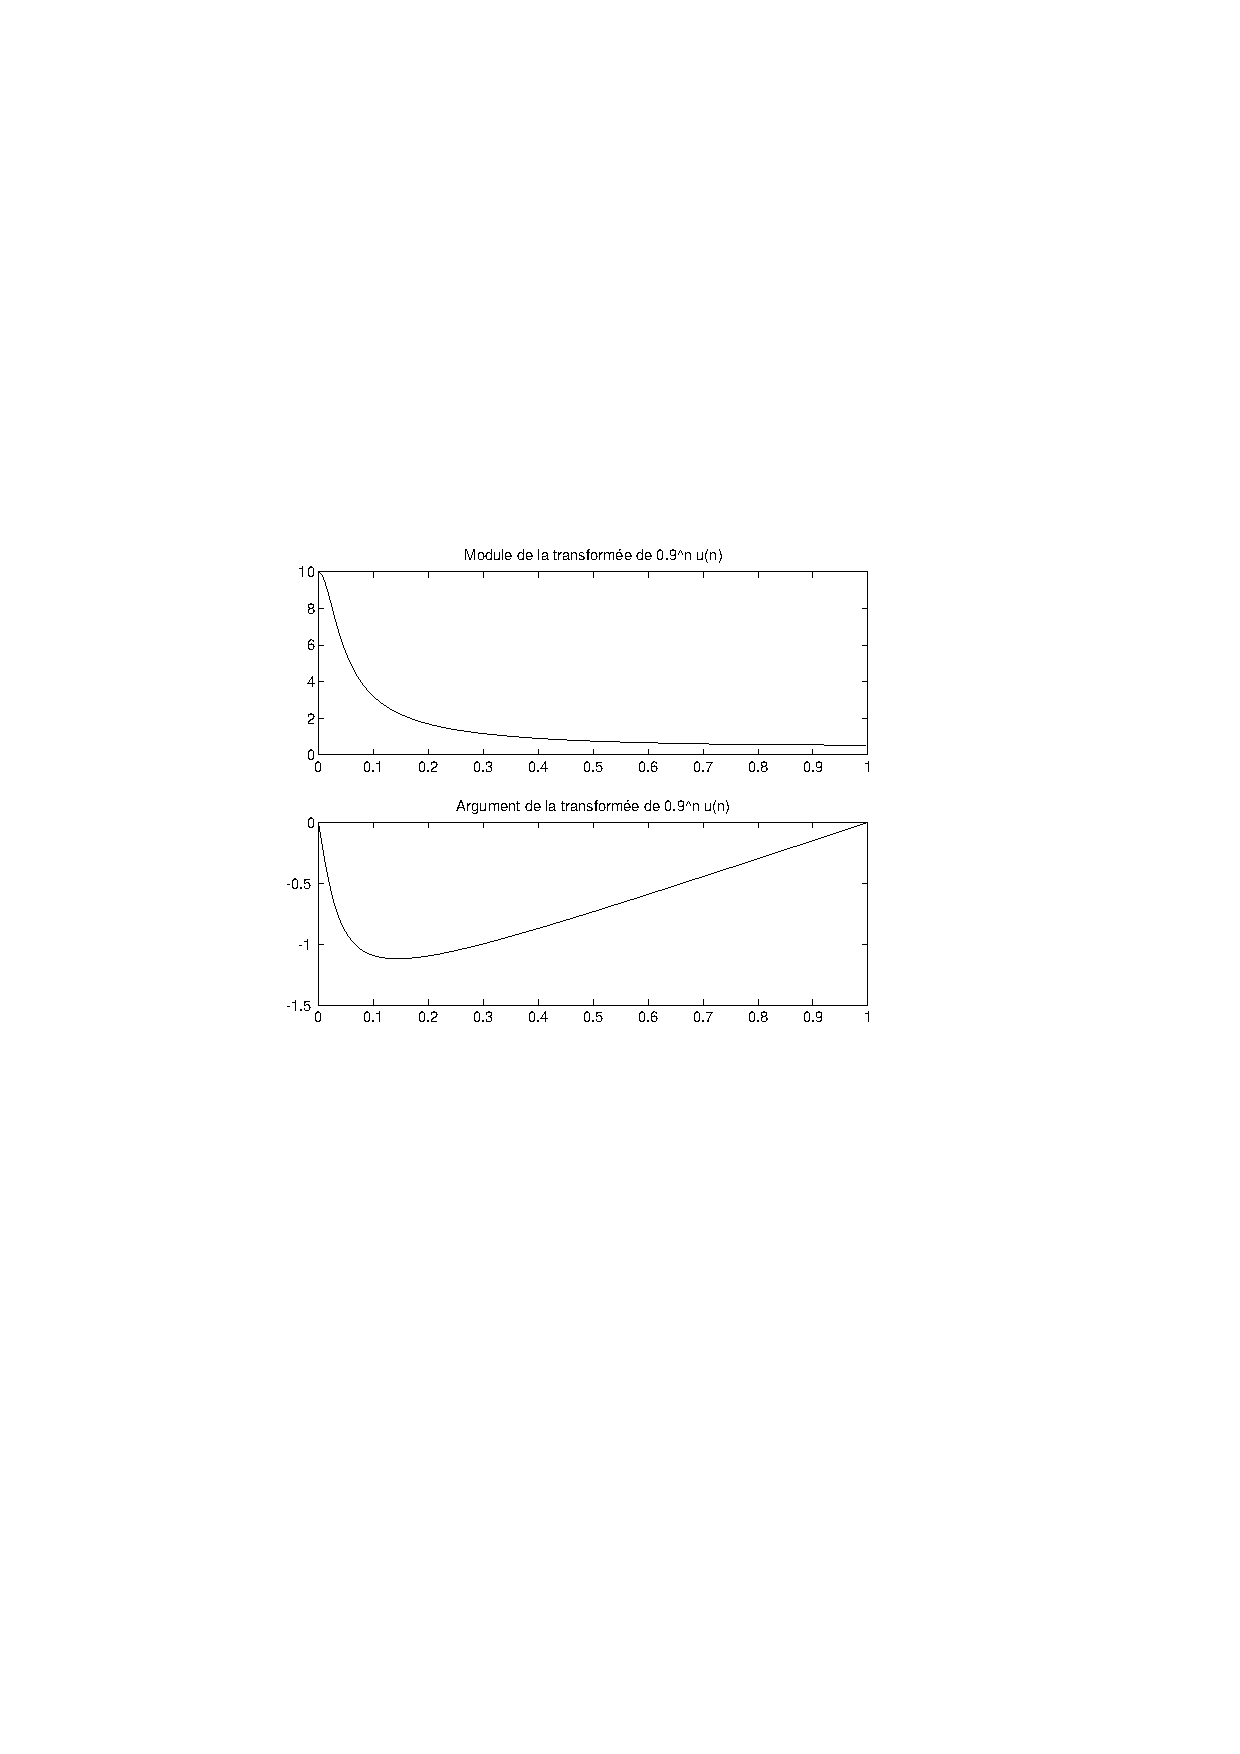
\includegraphics[width=0.6\textwidth]{Figures/FigMignotte-2}\\
  \caption{Transform\'{e}e de Fourier, module en haut, argument en bas, de $h_n= a^n \1_\nset(n)$ pour $a=0.9$
}\label{fig:FigMignotte-2}
\end{figure}
\section{Fonction de tranfert}
On a vu que la sortie $\sequence{v}[n][\nset]$ d'un système linéaire invariant dans le temps de r\'{e}ponse impulsionnelle $\sequence{h}[n][\nset]$ est donn\'{e}e par la convolution du signal d'entr\'{e}e $\sequence{u}[n][\nset]$ et de la réponse impulsionnelle $\sequence{h}[n][\nset]$, \ie\ 
$v_nj = (h * x)_n$ pour tout $n \in \zset$. La transformée en $z$ d'un produit de convolution étant égal au produit des transformées (la région de convergence étant l'intersection des régions de convergence de $U(z)$ et $H(z)$), nous avons donc
$$
V(z)=H(z)U(z) \eqsp.
$$
La transform\'{e}e en $z$, $H(z)$  de la r\'{e}ponse impulsionnelle $\sequence{h}[n][\zset]$ porte le nom de \emph{fonction de transfert} du syst\`{e}me lin\'{e}aire invariant. Cette transform\'{e}e en $z$, \'{e}valu\'{e}e sur le cercle de rayon unit\'{e} donne la transform\'{e}e de Fourier $H(\rme^{2 \rmi \pi \nu})$ de cette r\'{e}ponse impulsionnelle porte le nom de \emph{transmittance du syst\`{e}me} (on utilise aussi 
fonction de transfert pour cette quantité, bien que cette terminologie soit un peu incorrecte).

\subsection{Causalité et Stabilité}
\begin{definition}[SLI causal]
On dit qu'un système linéaire invariant dans le temps est causal si $h_n=0$ pour $n < 0$ où $\sequence{h}[n][\zset]$ est sa réponse impulsionnelle 
\end{definition}
On a vu que la région de convergence de la transform\'{e}e en $z$ d'une suite causale $\sequence{h}[n][\nset^]$ 
est une couronne  $\ensemble{z \in \cset}{|z| \geq \limsup_{n \to \infty} |h_n|^{1/n}= R_-}$. Comme par définition
une transform\'{e}e $H(p)= \infty$ lorsque $z= p$ est un pôle, une suite est causale si et seulement si
tous les p\^{o}les sont n\'{e}cessairement contenus \`{a} l'int\'{e}rieur d'un disque.

\begin{proposition}
la fonction de transfert d'un syst\`{e}me causal (c'est-\`{a}-dire dont la r\'{e}ponse impulsionnelle est causale) a ses p\^{o}les \`{a} l'int\'{e}rieur d'un cercle.
\end{proposition}

\begin{definition}[SLI stable]
un syst\`{e}me linéaire invariant dans le temps est stable si sa r\'{e}ponse impulsionnelle $\sequence{h}[n][\nset]$ est absolument sommable, 
$$
\sum_{n=-\infty}^{\infty}|h_n|<\infty \eqsp.
$$
\end{definition}
Or,
$$
|H(z)|=|\sum_{n=-\infty}^{\infty}h_n z^{-n}|\leq\sum_{n=-\infty}^{\infty}|h_nz^{-n}|
$$
et sur le cercle de rayon unit\'{e},
$$
|H(\rme^{2 \rmi \pi \nu})|=|\sum_{n=-\infty}^{\infty} |h_n|
$$
et si le dernier terme est born\'{e}, cela signifie bien que la transform\'{e}e de Fourier à temps-discret existe.  Donc, pour que le syst\`{e}me soit stable, le cercle de rayon unit\'{e} doit être inclus dans la région de convergence de la fonction de transfert qui est un anneau en toute g\'{e}n\'{e}ralit\'{e}.

Pour qu'un syst\`{e}me soit causal et stable, il faut que le cercle de rayon unit\'{e} appartienne au domaine de convergence, qui pour réponse causale est la couronne $\ensemble{z \in \cset}{|z| \geq R_-}$. Compte tenu de ce qui a \'{e}t\'{e} dit pr\'{e}c\'{e}demment, les p\^{o}les du syst\`{e}me doivent donc \^{e}tre contenus dans un disque $\ensemble{z \in \cset}{|z| < R}$ avec $R < 1$. 

\subsection{Equations aux diff\'{e}rences}
Lorsque le syst\`{e}me est r\'{e}gi par une \'{e}quation aux diff\'{e}rences du type
$$
\sum_{l=0}^{L}a_{l}y_{n-l}=\sum_{m=0}^{M}b_{m}x_{n-m}
$$
o\`{u} $\sequence{x}[n][\zset]$ et $\sequence{y}[n][\zset]$ sont les suites d'entr\'{e}e (excitation) et de sortie (r\'{e}ponse), on peut obtenir la r\'{e}ponse de r\'{e}gime en passant par la transform\'{e}e en $z$ bilat\'{e}rale. En utilisant les propri\'{e}t\'{e}s de lin\'{e}arit\'{e} et d\'{e}calage, on trouve finalement
\begin{equation}
\label{eq:tz-equation-difference}
Y(z)\sum_{l=0}^{L}a_{l}z^{-l}=X(z)\sum_{m=0}^{M}b_{m}z^{-m}
\end{equation}
On en d\'{e}duit que la fonction de transfert $G(z)$ s'\'{e}crit
$$
G(z)=\frac{\sum^{M}b_{m}z^{-m}}{\sum_{l=0}b_{l}z^{-l}} \eqsp.
$$
Cette fonction de transfert peut encore se mettre sous la forme
$$
\prod^{M}(1-z_{m}z^{-1})
$$
$$
G(z)=G_{0}\frac{m=1}{N}\text{   }(2.110)
$$
$$
\prod_{n=1}(1-p_{n}z^{-1})
$$
avec $G_{0}=\displaystyle \lim_{z\rightarrow\infty}G(z)$ . Pour trouver la r\'{e}ponse impulsionnelle, il suffit de d\'{e}- composer cette \'{e}quation en fractions simples et d'inverser ces derni\`{e}res.

A ce stade-ci, la r\'{e}gion de convergence de la transform\'{e}e n'est pas pr\'{e}cis\'{e}e.


